\documentclass[11pt,a4paper]{article}

% Packages
\usepackage[utf8]{inputenc}
\usepackage[T1]{fontenc}

\usepackage{geometry}
\usepackage{hyperref}
\usepackage{xcolor}
\usepackage{amsmath,amssymb}
\usepackage{array}
\usepackage{booktabs}
\usepackage{longtable}
\usepackage{tabularx}
\usepackage{enumitem}
\usepackage{float}
\usepackage{caption}
\usepackage{subcaption}
\usepackage{listings}
\usepackage{fancyhdr}
\usepackage{titlesec}
\usepackage{tcolorbox}
\usepackage{tikz}
\usetikzlibrary{arrows.meta,positioning,shapes.geometric,fit,backgrounds,calc}

\geometry{left=1in,right=1in,top=1.0in,bottom=1.0in}

% Colors
\definecolor{deepblue}{HTML}{16324F}
\definecolor{midblue}{HTML}{2B5C88}
\definecolor{lightblue}{HTML}{3A7CA5}
\definecolor{softblue}{HTML}{EAF3FA}
\definecolor{softgreen}{HTML}{E9F6EC}
\definecolor{softyellow}{HTML}{FFF8E1}
\definecolor{softred}{HTML}{FDECEC}
\definecolor{softgray}{HTML}{F6F7F9}
\definecolor{darkgray}{HTML}{333333}
\definecolor{codebg}{HTML}{F7F7F7}
\definecolor{coderule}{HTML}{D9DDE3}
\definecolor{promptbg}{HTML}{F0F4FF}
\definecolor{promptframe}{HTML}{4A6FA5}

% Section formatting
\titleformat{\section}{\Large\bfseries\color{deepblue}}{\thesection}{0.8em}{}
\titleformat{\subsection}{\large\bfseries\color{midblue}}{\thesubsection}{0.8em}{}
\titleformat{\subsubsection}{\normalsize\bfseries\color{lightblue}}{\thesubsubsection}{0.8em}{}

% Header / footer
\pagestyle{fancy}
\fancyhf{}
\fancyhead[L]{\small\textit{Orthosolver Lean Engine Architecture v2.1}}
\fancyhead[R]{\small\textit{Formalization, Repair, and Verification}}
\fancyfoot[C]{\small\thepage}
\renewcommand{\headrulewidth}{0.4pt}

% Hyperlinks
\hypersetup{colorlinks=true,linkcolor=deepblue,citecolor=deepblue,urlcolor=lightblue}

% tcolorbox
\tcbuselibrary{skins,breakable}
\newtcolorbox{mustbox}[1][] {colback=softred,colframe=red!60!black,fonttitle=\bfseries,title=#1,arc=2mm,boxrule=0.8pt,breakable}
\newtcolorbox{notebox}[1][] {colback=softblue,colframe=deepblue,fonttitle=\bfseries,title=#1,arc=2mm,boxrule=0.8pt,breakable}
\newtcolorbox{goodbox}[1][] {colback=softgreen,colframe=green!50!black,fonttitle=\bfseries,title=#1,arc=2mm,boxrule=0.8pt,breakable}
\newtcolorbox{policybox}[1][] {colback=softyellow,colframe=orange!70!black,fonttitle=\bfseries,title=#1,arc=2mm,boxrule=0.8pt,breakable}
\newtcolorbox{promptbox}[1][] {colback=promptbg,colframe=promptframe,fonttitle=\bfseries\color{white},colbacktitle=promptframe,title=#1,arc=2mm,boxrule=0.8pt,breakable}

% Listings
\lstdefinelanguage{json}{
  basicstyle=\ttfamily\small, numbers=left, numberstyle=\tiny\color{gray}, stepnumber=1, numbersep=8pt, showstringspaces=false, breaklines=true, frame=single, rulecolor=\color{coderule}, backgroundcolor=\color{codebg},
  literate=*{0}{{{0}}}{1}{1}{{{1}}}{1}{2}{{{2}}}{1}{3}{{{3}}}{1}{4}{{{4}}}{1}{5}{{{5}}}{1}{6}{{{6}}}{1}{7}{{{7}}}{1}{8}{{{8}}}{1}{9}{{{9}}}{1}{:}{{{\color{black}{:}}}}{1}{,}{{{\color{black}{,}}}}{1}{\{}{{{\color{black}{\{}}}}{1}{\}}{{{\color{black}{\}}}}}{1}{[}{{{\color{black}{[}}}}{1}{]}{{{\color{black}{]}}}}{1},
  morestring=[b]", stringstyle=\color{midblue}, commentstyle=\color{gray}, keywordstyle=\color{deepblue}\bfseries
}
\lstdefinelanguage{prompt}{basicstyle=\ttfamily\small,showstringspaces=false,breaklines=true,frame=none,backgroundcolor=\color{promptbg},columns=flexible}
\lstdefinelanguage{hcl}{
  basicstyle=\ttfamily\small, numbers=left, numberstyle=\tiny\color{gray}, stepnumber=1, numbersep=8pt, showstringspaces=false, breaklines=true, frame=single, rulecolor=\color{coderule}, backgroundcolor=\color{codebg},
  keywords={resource,variable,output,data,locals,module,provider,terraform,required_providers,backend,for_each,count,depends_on,lifecycle,dynamic,content},
  keywordstyle=\color{deepblue}\bfseries, morestring=[b]", stringstyle=\color{midblue}, morecomment=[l]{\#}, commentstyle=\color{gray}\itshape, columns=flexible
}
\lstset{language=json}

\newcommand{\Lean}{\textsc{Lean}}
\newcommand{\Vertex}{Vertex AI}
\newcommand{\Claude}{Claude}

\begin{document}

\begin{titlepage}
\centering
\vspace*{1.6cm}

{\Huge\bfseries\color{deepblue} Orthosolver Lean Engine \\[0.3cm] Architecture Specification}

\vspace{0.8cm}

{\Large\color{midblue} Formalization, Compilation, Repair Loop, \\[0.15cm] and Failure Classification}

\vspace{0.7cm}
\rule{0.75\textwidth}{1pt}

\vspace{1.0cm}

{\large Implementation Specification for the Lean Engine Engineer}

\vspace{0.4cm}

{\normalsize Version 2.1 \\ March 2026}

\vspace{1.5cm}

\begin{abstract}
\noindent This document specifies the complete architecture of the Orthosolver \Lean{} engine: the four operating modes (assembly check, lemma formalization, root assembly, statement plausibility check), the internal \Claude{} formalization agent (Agent~6), the statement plausibility checker (Agent~7), the hybrid stateful/stateless repair loop, the error classification taxonomy, the Docker environment with pre-compiled Mathlib, and the HTTP API contract the engine must implement. This document also describes what the NL pipeline sends to the engine and how it uses results, so the engine engineer has full context. It does \textbf{not} specify the NL agents (1--5), the controller routing logic, or the database schema. Those are in the companion document: \textit{Orthosolver NL Pipeline Architecture Specification}.
\end{abstract}

\vfill

{\small Companion document: \textit{Orthosolver NL Pipeline Architecture Specification v2.1}}
\end{titlepage}

\tableofcontents
\newpage

%% ═══════════════════════════════════════════════════════════════════════════════
\section{Purpose, Audience, and Scope}
%% ═══════════════════════════════════════════════════════════════════════════════

This document is for the engineer implementing the \Lean{} engine service. It contains everything needed to build, test, and deploy the engine as a standalone service that exposes the HTTP API contract defined in Section~\ref{sec:api_contract}.

\subsection{What This Document Covers}
\begin{itemize}[leftmargin=2em]
  \item The four \Lean{} engine modes and their detailed behavior.
  \item The internal repair loop (hybrid stateful/stateless conversation model).
  \item Complete agent prompt specifications for Agent 6 (formalization) and Agent 7 (plausibility checker).
  \item The full error classification taxonomy and what each class means.
  \item The HTTP API contract the engine must implement.
  \item What the NL pipeline sends and how it uses results (integration context).
  \item The \Lean{} Docker environment with pre-compiled Mathlib.
  \item Lean-engine-specific GCP deployment and Terraform.
\end{itemize}

\subsection{What This Document Does \textbf{Not} Cover}
\begin{itemize}[leftmargin=2em]
  \item NL agent prompts (Agents 1--5), controller routing tables, database DDL, public API.
  \item These are in the companion doc: \textit{Orthosolver NL Pipeline Architecture Specification}.
\end{itemize}

%% ═══════════════════════════════════════════════════════════════════════════════
\section{System Context: Where the Lean Engine Fits}
%% ═══════════════════════════════════════════════════════════════════════════════

\subsection{High-Level Flow}

The Orthosolver system has two halves: a natural-language pipeline (orchestrator + NL agents) and the \Lean{} engine (this service). The NL pipeline handles decomposition, proof search, and vetting. It calls the \Lean{} engine as a black-box service when it needs formal verification.

\begin{figure}[H]
\centering
\resizebox{0.85\textwidth}{!}{%
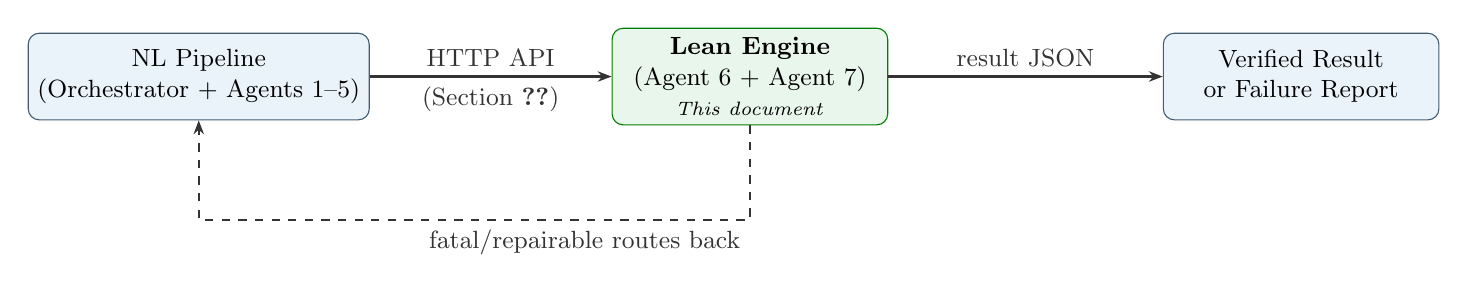
\begin{tikzpicture}[
  every node/.style={font=\small},
  comp/.style={rectangle,rounded corners=4pt,draw=deepblue!80,fill=softblue,minimum width=3.5cm,minimum height=1.1cm,align=center},
  lean/.style={rectangle,rounded corners=4pt,draw=green!50!black,fill=softgreen,minimum width=3.5cm,minimum height=1.1cm,align=center},
  arrow/.style={-{Stealth[length=5pt]},thick,color=darkgray}
]
\node[comp] (nl) at (0,0) {NL Pipeline\\(Orchestrator + Agents 1--5)};
\node[lean] (le) at (7,0) {\textbf{Lean Engine}\\(Agent 6 + Agent 7)\\{\scriptsize \textit{This document}}};
\node[comp] (result) at (14,0) {Verified Result\\or Failure Report};

\draw[arrow] (nl) -- node[above]{\small HTTP API} node[below]{\small (Section~\ref{sec:api_contract})} (le);
\draw[arrow] (le) -- node[above]{\small result JSON} (result);
\draw[arrow,dashed] (le.south) -- ++(0,-1.2) -| node[pos=0.15,below]{\small fatal/repairable routes back} (nl.south);
\end{tikzpicture}%
}
\caption{The \Lean{} engine is a standalone service. The NL pipeline calls it via HTTP and routes on the result.}
\end{figure}

\subsection{What the NL Pipeline Sends You}

The orchestrator constructs a job request containing:

\begin{itemize}[leftmargin=2em]
  \item \textbf{A mode} (\texttt{check\_assembly}, \texttt{formalize\_lemma}, \texttt{assemble\_root}, or \texttt{check\_statement\_plausibility}).
  \item \textbf{Natural-language statement(s)} with structured semantic sketches (JSON objects capturing variables, quantifier order, domain restrictions, witness dependencies).
  \item \textbf{Natural-language proof} (for \texttt{formalize\_lemma}).
  \item \textbf{Pinned statement signature} (for \texttt{formalize\_lemma}): the \Lean{} type signature that your output declaration \textbf{must} match exactly.
  \item \textbf{Trusted formal context}: previously compiled \Lean{} declarations you may use.
  \item \textbf{Assembly plan} (for \texttt{check\_assembly} and \texttt{assemble\_root}): how lemmas combine.
  \item \textbf{Budget parameters}: max repair rounds, max tool calls, timeout.
\end{itemize}

\subsection{How the NL Pipeline Uses Your Results}

The orchestrator routes on your \texttt{status} and \texttt{error\_class}:

\begin{itemize}[leftmargin=2em]
  \item \texttt{success} $\to$ declaration enters trusted context. Orchestrator proceeds.
  \item \texttt{repairable} with Lean-only class (\texttt{syntax}, \texttt{type\_mismatch}, \texttt{missing\_import}) $\to$ orchestrator re-dispatches to you with same input.
  \item \texttt{repairable} with NL-loop class (\texttt{tactic\_failure}, \texttt{missing\_library\_fact}) $\to$ one more \Lean{} attempt, then orchestrator sends lemma back to NL solver with your diagnostics.
  \item \texttt{fatal/false\_lemma\_suspected} $\to$ orchestrator runs plausibility check, then may invalidate decomposition.
  \item \texttt{fatal/major\_proof\_gap} $\to$ orchestrator decomposes the lemma further or retries NL.
  \item \texttt{fatal/assembly\_composition\_failure} $\to$ orchestrator retries assembly plan, not individual lemmas.
\end{itemize}

Your \texttt{recommended\_next\_step} and \texttt{routing\_confidence} help the orchestrator choose, but the orchestrator makes the final routing decision.

\subsection{NL-Only Mode}
When the orchestrator runs in NL-only mode, it never contacts the \Lean{} engine at all. No jobs will arrive. The engine does not need to be aware of this mode; it simply receives no traffic.

%% ═══════════════════════════════════════════════════════════════════════════════
\section{Key Concepts}
%% ═══════════════════════════════════════════════════════════════════════════════

\subsection{Semantic Sketch}
A structured JSON object attached to every theorem and lemma. Not a \Lean{} formalization, but precise enough for drift detection. Contains: typed variables, quantifier order, domain restrictions, witness dependencies, normalized claim.

\begin{lstlisting}
{
  "variables": [ {"name": "f", "type": "function R -> R", "domain": "[0,1]"} ],
  "quantifier_order": ["forall n", "exists C"],
  "domain_restrictions": ["n >= 1", "f continuous"],
  "witness_dependencies": ["C depends on n and f"],
  "normalized_claim": "string"
}
\end{lstlisting}

\subsection{Pinned Statement Signatures}
During \texttt{check\_assembly}, the engine formalizes each lemma statement and produces a \Lean{} type signature. These are returned to the orchestrator and stored. When \texttt{formalize\_lemma} is dispatched, the pinned signature is included in the request. The engine \textbf{must} produce a declaration whose type matches the pinned signature exactly.

\subsection{Trusted Formal Context}
The set of \Lean{} declarations that have already compiled successfully in earlier jobs for this problem. The orchestrator sends them in the job request. The engine may use them via \texttt{import} or direct reference. The engine must not modify or contradict them.

\subsection{Assembly Plan}
A structured plan showing how lemma declarations combine to prove the root theorem. Each step cites lemma names and states what follows trivially. The engine must be able to close the assembly proof using only the cited declarations and trivial composition.

%% ═══════════════════════════════════════════════════════════════════════════════
\section{Lean Engine Modes}
\label{sec:modes}
%% ═══════════════════════════════════════════════════════════════════════════════

The engine supports four modes. Externally it is a single API; internally each mode has different behavior.

\subsection{Mode: \texttt{check\_assembly}}

\textbf{Purpose:} Verify that the decomposition structure is formally sound before the orchestrator invests in full proof formalization.

\textbf{Behavior:}
\begin{enumerate}[leftmargin=2em]
  \item Formalize the root theorem statement as a \Lean{} proposition.
  \item Formalize each lemma statement as an \texttt{axiom} (assumed declaration) in a scratch file.
  \item Formalize the assembly plan skeleton: write a proof of the root theorem that cites only the assumed declarations and applies trivial composition.
  \item Run \texttt{lake build}. If it compiles, the assembly structure is sound.
  \item On success: extract the \Lean{} type signature of each assumed declaration and return them as \texttt{pinned\_statement\_signatures}.
  \item On failure: attempt repair up to \texttt{max\_repair\_rounds}. Classify failure.
\end{enumerate}

At most \texttt{assembly\_check\_repair\_rounds} repair rounds. At most \texttt{max\_tool\_calls} tool calls.

\subsection{Mode: \texttt{formalize\_lemma}}

\textbf{Purpose:} Produce a compiling \Lean{} 4 theorem and proof for a single lemma.

\textbf{Behavior:}
\begin{enumerate}[leftmargin=2em]
  \item Receive NL statement, NL proof, semantic sketch, pinned signature, and trusted context.
  \item The declaration header \textbf{must} match the pinned signature exactly. Do not change the type.
  \item Translate the NL proof to \Lean{} tactics, mapping each proof step to a tactic.
  \item Run \texttt{lake build}. If success, done.
  \item If failure, run the repair loop (Section~\ref{sec:repair_loop}).
  \item Classify the terminal state as \texttt{success}, \texttt{repairable}, or \texttt{fatal}.
\end{enumerate}

The engine is the authority on whether a repair failure is mathematical (the NL proof is wrong) or a formalization artifact (syntax, missing library lemma).

\subsection{Mode: \texttt{assemble\_root}}

\textbf{Purpose:} Prove the root theorem by composing real compiled declarations (not assumptions).

\textbf{Dispatched only when:} All required lemmas have compiled successfully and their declarations are in trusted context.

\textbf{Behavior:}
\begin{enumerate}[leftmargin=2em]
  \item Receive actual compiled declaration names (not axioms) and the assembly plan.
  \item Write a proof of the root theorem that imports trusted context and applies trivial composition.
  \item Run \texttt{lake build}. The proof must compile with no \texttt{sorry} or \texttt{admit}.
\end{enumerate}

\begin{goodbox}[On \texttt{assembly\_composition\_failure}]
If \texttt{assemble\_root} fails with individually-valid declarations that do not compose due to type-level mismatches, return \texttt{assembly\_composition\_failure}. The lemmas are NOT wrong (they are still in trusted context). The orchestrator will retry with a revised assembly plan.
\end{goodbox}

\subsection{Mode: \texttt{check\_statement\_plausibility}}

\textbf{Purpose:} Lightweight falsifiability check. No proof search. Hard timeout.

\textbf{Behavior:}
\begin{enumerate}[leftmargin=2em]
  \item Formalize the statement as a \Lean{} proposition (type-check: is it well-typed?).
  \item Attempt to prove \texttt{False} from the statement using only: \texttt{norm\_num}, \texttt{decide}, \texttt{simp}, \texttt{native\_decide}.
  \item Do NOT attempt non-trivial tactics beyond those four.
  \item Stop after timeout regardless of result.
\end{enumerate}

Returns: \texttt{plausible} (well-typed, not refuted), \texttt{suspected\_false} (refuted), or \texttt{inconclusive} (could not type-check or timed out).

%% ═══════════════════════════════════════════════════════════════════════════════
\section{Internal Repair Loop}
\label{sec:repair_loop}
%% ═══════════════════════════════════════════════════════════════════════════════

The repair loop uses a \textbf{hybrid stateful/stateless} conversation model with Agent~6 (\Claude{} running through \Vertex{}).

\subsection{Stateful Phase}
Within a single repair session, the conversation is stateful. Agent~6 accumulates:
\begin{itemize}[leftmargin=2em]
  \item The current scratch \texttt{.lean} file contents.
  \item Compiler diagnostics from each \texttt{build()} call.
  \item A log of attempted tactics and their outcomes.
  \item Search results from \texttt{search\_mathlib()} calls.
\end{itemize}

\subsection{Context Compression}
When the conversation approaches \texttt{repair\_context\_token\_budget}, the engine summarizes the repair history into a compressed state object (current file, key diagnostics, what has been tried) and starts a \textbf{fresh context} with that summary. This prevents context window overflow while preserving essential repair history.

\subsection{Between Jobs}
Between separate \Lean{} jobs for the same lemma (e.g., after the NL pipeline produces a new proof), the context is always fresh. No state carries over from a previous job.

\subsection{Tool Interface}

Agent~6 has access to these tools during the repair loop:

\begin{itemize}[leftmargin=2em]
  \item \texttt{write\_file(path, content)}: Write or overwrite the scratch \Lean{} file.
  \item \texttt{build()}: Invoke \texttt{lake build} and return compiler diagnostics.
  \item \texttt{get\_goal(line, column)}: Query proof state at a position in the file.
  \item \texttt{search\_mathlib(query)}: Search Mathlib for relevant declarations.
  \item \texttt{read\_file(path)}: Read a file in the project.
\end{itemize}

\subsection{Repair Round Budget}

Each call to \texttt{build()} after the first counts as one repair round. The engine stops when: (a) \texttt{build()} succeeds, (b) \texttt{max\_repair\_rounds} is reached, (c) \texttt{max\_tool\_calls\_per\_job} is reached, or (d) \texttt{timeout\_seconds} is reached. On hitting any limit without success, Agent~6 must classify the failure and produce the terminal result JSON.

%% ═══════════════════════════════════════════════════════════════════════════════
\section{Error Classification Taxonomy}
\label{sec:errors}
%% ═══════════════════════════════════════════════════════════════════════════════

The engine must classify every non-success outcome into one of three categories and one of twelve error classes. This classification drives the orchestrator's routing decisions.

\subsection{Three Categories}

\begin{itemize}[leftmargin=2em]
  \item \texttt{success}: \texttt{build()} returned no errors. The declaration compiles.
  \item \texttt{repairable}: The repair limit was hit but more rounds could close it. The gap is a formalization artifact, not a mathematical problem.
  \item \texttt{fatal}: A fundamental issue that more repair rounds cannot fix.
\end{itemize}

\subsection{Twelve Error Classes}

\subsubsection{Repairable --- Lean-Only Retry}

These are formalization artifacts. No mathematical gap. The orchestrator re-dispatches to the engine directly.

\begin{itemize}[leftmargin=2em]
  \item \texttt{syntax}: Lean syntax errors (parentheses, keywords, indentation).
  \item \texttt{type\_mismatch}: Type errors that can be resolved with explicit casts or signature adjustments.
  \item \texttt{missing\_import}: A needed Mathlib import is not present.
\end{itemize}

\subsubsection{Repairable --- NL Loop Needed}

The gap may indicate the NL proof's reasoning does not map cleanly to available Mathlib API. After one more engine attempt, the orchestrator will return to NL solver with diagnostics.

\begin{itemize}[leftmargin=2em]
  \item \texttt{tactic\_failure}: A tactic fails and no alternative closes the goal. The NL proof step may need different justification.
  \item \texttt{missing\_library\_fact}: The proof relies on a fact that does not exist in Mathlib at the pinned version.
\end{itemize}

\subsubsection{Fatal}

\begin{itemize}[leftmargin=2em]
  \item \texttt{false\_lemma\_suspected}: Evidence that the lemma statement is false (e.g., a counterexample was found during formalization, or the formalized negation was proved).
  \item \texttt{major\_proof\_gap}: The NL proof has a step that cannot be formalized because it is mathematically unjustified. Not a syntax or library issue.
  \item \texttt{assembly\_invalid}: (assembly modes only) The assembly skeleton does not compile even with assumed declarations.
  \item \texttt{assembly\_composition\_failure}: (\texttt{assemble\_root} only) Individual declarations are valid but do not compose due to type-level incompatibilities.
  \item \texttt{bad\_statement\_translation}: The NL statement is too ambiguous to produce a well-typed \Lean{} proposition.
  \item \texttt{environment\_mismatch}: The requested \texttt{lean\_image\_tag} does not match the engine's baked version.
  \item \texttt{unknown\_fatal}: None of the above. Should be rare. Include detailed diagnostics.
\end{itemize}

\subsection{Error Scope}

Each error also carries a \texttt{scope}: \texttt{statement} (the formalized statement is the problem), \texttt{proof} (the proof body), \texttt{assembly} (the composition step), \texttt{environment} (infrastructure / toolchain), or \texttt{infrastructure} (parse errors, timeouts, etc.).

\begin{mustbox}[Classification Accuracy Is Critical]
The orchestrator trusts the engine's classification to make routing decisions. Misclassifying a mathematical gap as a formalization artifact wastes \Lean{} retries. Misclassifying a formalization artifact as fatal wastes NL retries or destroys valid decompositions. When uncertain, prefer \texttt{repairable} with NL-loop class to give the orchestrator room to decide.
\end{mustbox}

%% ═══════════════════════════════════════════════════════════════════════════════
\section{Agent Prompt Specifications}
\label{sec:prompts}
%% ═══════════════════════════════════════════════════════════════════════════════

\subsection{Agent 6: Lean Engine Formalization Agent}

\textbf{When called:} Inside the repair loop. This is the \Claude{} agent running in a stateful multi-turn conversation within a single repair session. It has tool access to read/write \Lean{} files, invoke \texttt{lake build}, query compiler diagnostics, and search library declarations.

\textbf{Purpose:} Translate NL statements and proofs into compiling \Lean{} 4 code. Repair compiler errors iteratively. Classify failures accurately.

\begin{promptbox}[Agent 6 System Prompt: Lean Engine Formalization Agent]
\begin{lstlisting}[language=prompt]
You are an expert Lean 4 / Mathlib formalization engineer. Your job
is to produce a complete, compiling Lean 4 theorem and proof.

You will be given:
- A natural-language lemma statement and its semantic sketch
- A natural-language proof
- A pinned Lean statement signature (you MUST produce a declaration
  that matches this signature exactly -- do not change the type)
- The formal environment: previously compiled declarations you may
  use directly
- The current scratch .lean file contents and latest compiler output
  (on repair rounds)

Your tools:
- write_file(path, content): write or overwrite the scratch file
- build(): invoke lake build and return compiler diagnostics
- get_goal(line, column): query proof state at a position
- search_mathlib(query): search Mathlib for relevant declarations
- read_file(path): read a file

Workflow:
1. Study the natural-language proof to understand the proof
   strategy.
2. Translate the STATEMENT first. The declaration header MUST
   match the pinned signature exactly.
3. Translate the PROOF. Map each NL proof step to a tactic.
4. Call build(). If it succeeds, you are done.
5. If it fails, read the diagnostics carefully.
   - Distinguish formalization difficulty (syntax, type errors,
     missing lemmas) from mathematical gaps (a step that cannot
     be formalized because the NL proof is wrong).
   - For formalization issues: search_mathlib(), adjust tactics,
     try alternatives (ring, simp, linarith, omega, norm_num,
     field_simp, exact?, apply?).
   - For mathematical gaps: do NOT invent a sorry. Report the
     gap accurately in your final output.
6. Repeat up to the configured max_repair_rounds.

Classification rules (for your final output):
- "success": build() returned no errors.
- "repairable": you hit the repair limit but believe more rounds
  would close it (formalization difficulty only, no math gap).
  error_class must be one of: syntax, type_mismatch,
  missing_import, tactic_failure, missing_library_fact.
- "fatal/major_proof_gap": the NL proof has a step that cannot be
  formalized because it is mathematically unjustified.
- "fatal/false_lemma_suspected": you found evidence the statement
  is false while attempting to formalize.
- "fatal/bad_statement_translation": the NL statement is too
  ambiguous to produce a well-typed Lean proposition.
- "fatal/assembly_composition_failure": (assemble_root mode only)
  the individual declarations do not compose due to type-level
  incompatibilities.

Never use sorry, admit, or native_decide as a shortcut for a proof
step. Never inject a false theorem into context.

After each build() call, report your current status in JSON.
When you have reached a terminal state (success or fatal), output
the final JSON result and stop.

You must output ONLY valid JSON as your final message.
\end{lstlisting}
\end{promptbox}

\textbf{Final output schema (terminal state):}
\begin{lstlisting}
{
  "status": "success | repairable | fatal",
  "mode": "formalize_lemma | check_assembly | assemble_root | check_statement_plausibility",
  "decl_name": "string or null",
  "lean_code": "string or null",
  "compiler_ok": true,
  "repair_rounds_used": 0,
  "error_class": "string or null",
  "error_scope": "statement | proof | assembly | environment | null",
  "error_message": "string or null",
  "diagnostics": [
    { "severity": "error | warning", "message": "string", "line": 0, "column": 0 }
  ],
  "math_gap_description": "string or null",
  "recommended_next_step": "accept | retry_lean_only | retry_nl_proof | decompose_current | invalidate_parent_decomposition | retry_assembly_plan",
  "routing_confidence": 0.0
}
\end{lstlisting}

\subsection{Agent 7: Statement Plausibility Checker}

\textbf{When called:} Inside the \texttt{check\_statement\_plausibility} mode. This is a lightweight agent with a hard timeout.

\begin{promptbox}[Agent 7 System Prompt: Statement Plausibility Checker]
\begin{lstlisting}[language=prompt]
You are a Lean 4 falsifiability checker. Your ONLY job is to
determine whether a mathematical statement is immediately
falsifiable using simple automated tactics.

You are NOT attempting to prove the statement. You are NOT doing
a full proof search. You have a hard time limit.

Procedure:
1. Formalize the statement as a Lean 4 proposition (type-check
   only -- does it produce a well-typed Prop?).
2. Attempt to prove False from the statement using:
   - norm_num
   - decide (for decidable propositions with small domains)
   - simp
   - native_decide (for decidable propositions)
3. Do NOT attempt any non-trivial tactic beyond the above four.
4. Stop after the time limit regardless of result.

Output exactly one of three verdicts:
- "plausible": well-typed and the above tactics could not refute.
- "suspected_false": a tactic produced a proof of False, or the
  statement is ill-typed revealing logical impossibility.
- "inconclusive": could not type-check, or tactics timed out.

You must output ONLY the following JSON object and nothing else.
\end{lstlisting}
\end{promptbox}

\textbf{Output schema:}
\begin{lstlisting}
{
  "status": "completed",
  "verdict": "plausible | suspected_false | inconclusive",
  "evidence": "string",
  "tactic_used": "string or null",
  "lean_code_attempted": "string or null",
  "confidence": 0.0
}
\end{lstlisting}

\subsection{Prompt Injection Contract}

Agent~6 is called in a stateful multi-turn conversation. Temperature 0 by default; may use 0.2 on repair retries for proof creativity. Agent~7 is a single-turn call with temperature 0.

All agent outputs stored verbatim as GCS artifacts before parsing. Parse failures retry once; second failure is \texttt{fatal/infrastructure}.

%% ═══════════════════════════════════════════════════════════════════════════════
\section{Lean Engine HTTP API Contract}
\label{sec:api_contract}
%% ═══════════════════════════════════════════════════════════════════════════════

This is the API the engine must implement. The orchestrator is the sole client.

\subsection{Service Identity and Networking}

The engine is deployed as a \textbf{private} Cloud Run service. Not exposed on \texttt{orthos-ai.com}. The orchestrator authenticates via GCP service-to-service IAM (Cloud Run invoker role, OIDC tokens).

\begin{lstlisting}
# Production (internal Cloud Run URL):
  https://orthos-lean-engine-<hash>-<region>.a.run.app/v1/...

# Local development:
  http://localhost:8081/v1/...
\end{lstlisting}

\subsection{Communication Model: Asynchronous with Polling}

Jobs are asynchronous. The orchestrator submits, then polls.

\begin{enumerate}[leftmargin=2em]
  \item Orchestrator POSTs \texttt{/v1/jobs} with job specification.
  \item Engine validates, enqueues, returns \texttt{202 Accepted} with \texttt{job\_id}.
  \item Orchestrator polls \texttt{GET /v1/jobs/\{job\_id\}} (recommended: 5s interval).
  \item On terminal state, poll response includes full result.
  \item Optional: POST webhook callback to \texttt{callback\_url}. Best-effort only.
\end{enumerate}

\subsection{Endpoints}

\subsubsection{POST \texttt{/v1/jobs} --- Submit Job}

\textbf{Request headers:}
\begin{lstlisting}
Content-Type: application/json
Authorization: Bearer <GCP_OIDC_TOKEN>
X-Request-Id: <uuid>
X-Idempotency-Key: <job_id>
\end{lstlisting}

\textbf{Request body:}
\begin{lstlisting}
{
  "job_id": "lean_job_lem_002_v1",
  "problem_id": "prob_20260311_001",
  "target_id": "lem_002",
  "target_kind": "lemma | theorem | assembly",
  "mode": "check_assembly | formalize_lemma | assemble_root | check_statement_plausibility",
  "lean_image_tag": "Orthosolver-lean-4.18.0-mathlib-v4.18.0",
  "callback_url": "string or null",
  "payload": { "... mode-specific ..." }
}
\end{lstlisting}

\textbf{Mode payloads:}

\paragraph{\texttt{check\_assembly}:}
\begin{lstlisting}
{
  "theorem_nl": "string",
  "theorem_semantic_sketch": {},
  "lemmas": [ { "local_id": "L1", "statement_nl": "string", "semantic_sketch": {} } ],
  "assembly_plan": { "steps": [], "proof_skeleton_nl": "string" },
  "imports": ["Mathlib"],
  "max_repair_rounds": 2, "max_tool_calls": 30, "timeout_seconds": 240
}
\end{lstlisting}

\paragraph{\texttt{formalize\_lemma}:}
\begin{lstlisting}
{
  "lemma_id": "lem_002",
  "statement_nl": "string",
  "semantic_sketch": {},
  "proof_nl": "string",
  "pinned_statement_signature": "theorem lemma_bound ...",
  "trusted_context": [ { "decl_name": "string", "lean_code": "string" } ],
  "imports": ["Mathlib"],
  "max_repair_rounds": 5, "max_tool_calls": 60,
  "timeout_seconds": 300, "repair_context_token_budget": 32000
}
\end{lstlisting}

\paragraph{\texttt{assemble\_root}:}
\begin{lstlisting}
{
  "theorem_nl": "string",
  "theorem_semantic_sketch": {},
  "assembly_plan": { "steps": [], "proof_skeleton_nl": "string" },
  "trusted_context": [ { "decl_name": "string", "lean_code": "string" } ],
  "imports": ["Mathlib"],
  "max_repair_rounds": 3, "max_tool_calls": 60, "timeout_seconds": 300
}
\end{lstlisting}

\paragraph{\texttt{check\_statement\_plausibility}:}
\begin{lstlisting}
{
  "statement_nl": "string",
  "semantic_sketch": {},
  "imports": ["Mathlib"],
  "timeout_seconds": 45
}
\end{lstlisting}

\textbf{Response (\texttt{202 Accepted}):}
\begin{lstlisting}
{
  "job_id": "lean_job_lem_002_v1",
  "status": "queued",
  "created_at": "2026-03-11T15:13:00Z",
  "estimated_duration_seconds": 120
}
\end{lstlisting}

\textbf{Error responses:} 400 (malformed), 409 (idempotency: returns existing job status), 422 (\texttt{lean\_image\_tag} mismatch), 503 (at capacity).

\subsubsection{Idempotency}

The engine must be idempotent on \texttt{job\_id} (via the \texttt{X-Idempotency-Key} header). If a job with that ID already exists, return its current status. Do not re-execute. This guarantees exactly-once semantics under at-least-once delivery.

\subsubsection{GET \texttt{/v1/jobs/\{job\_id\}} --- Poll Status}

\textbf{While running:}
\begin{lstlisting}
{
  "job_id": "lean_job_lem_002_v1",
  "status": "running",
  "mode": "formalize_lemma",
  "repair_rounds_used": 2,
  "elapsed_seconds": 87,
  "updated_at": "2026-03-11T15:14:27Z"
}
\end{lstlisting}

\textbf{Terminal state:}
\begin{lstlisting}
{
  "job_id": "lean_job_lem_002_v1",
  "status": "success | repairable | fatal",
  "mode": "formalize_lemma",
  "result": {
    "decl_name": "string or null",
    "lean_code": "string or null",
    "compiler_ok": true,
    "repair_rounds_used": 3,
    "pinned_statement_signatures": null,
    "error_class": "string or null",
    "error_scope": "statement | proof | assembly | environment | null",
    "error_message": "string or null",
    "diagnostics": [ { "severity": "error | warning", "message": "string", "line": 0, "column": 0 } ],
    "math_gap_description": "string or null",
    "recommended_next_step": "accept | retry_lean_only | retry_nl_proof | decompose_current | invalidate_parent_decomposition | retry_assembly_plan",
    "routing_confidence": 0.95
  },
  "created_at": "2026-03-11T15:13:00Z",
  "completed_at": "2026-03-11T15:15:42Z"
}
\end{lstlisting}

For \texttt{check\_assembly} success, \texttt{result} includes \texttt{pinned\_statement\_signatures}. For \texttt{check\_statement\_plausibility}, \texttt{result} uses \texttt{verdict}/\texttt{evidence}/\texttt{tactic\_used}/\texttt{confidence}.

\subsubsection{POST \texttt{/v1/jobs/\{job\_id\}/cancel}}
Cancel a running job. Graceful shutdown within timeout grace period.

\subsubsection{GET \texttt{/v1/health}}
\begin{lstlisting}
{
  "status": "healthy | degraded | overloaded",
  "lean_image_tag": "Orthosolver-lean-4.18.0-mathlib-v4.18.0",
  "active_jobs": 3,
  "max_concurrent_jobs": 8,
  "queue_depth": 1
}
\end{lstlisting}

\subsection{Webhook Callback}
If \texttt{callback\_url} is provided, POST the terminal result to that URL on completion. Retry up to 3 times with exponential backoff. Orchestrator must return 200 within 5 seconds. Best-effort only.

%% ═══════════════════════════════════════════════════════════════════════════════
\section{Lean Docker Environment}
%% ═══════════════════════════════════════════════════════════════════════════════

\subsection{Pre-Built Mathlib Image}

The engine runs on a Docker image with Mathlib pre-compiled at a pinned version. The image tag encodes both the \Lean{} version and the Mathlib version (e.g., \texttt{Orthosolver-lean-4.18.0-mathlib-v4.18.0}).

Each job writes a scratch \texttt{.lean} file and runs incremental \texttt{lake build} on top of the pre-built environment. No per-job Mathlib rebuild occurs; startup time is seconds, not minutes.

\subsection{Image Tag Enforcement}

The Mathlib version is set at problem creation and locked for that problem's lifetime. The engine \textbf{must reject} any job whose \texttt{lean\_image\_tag} does not match its baked version (return 422). Updating Mathlib requires deploying a new image tag; it does not affect in-flight problems.

\subsection{Scratch File Management}

Each job operates on an isolated scratch directory. The scratch file is written by Agent~6 via \texttt{write\_file()}. The final \texttt{.lean} file and \texttt{build.log} are stored as GCS artifacts.

\subsection{Resource Requirements}

The engine requires more CPU and memory than NL agents due to \Lean{} compilation:

\begin{itemize}[leftmargin=2em]
  \item CPU: 4 vCPUs per instance (recommended).
  \item Memory: 8 GiB per instance (Mathlib imports are memory-intensive).
  \item Disk: 10+ GiB for the pre-built Mathlib oleans.
  \item Timeout: up to 600s per request (Cloud Run max).
\end{itemize}

%% ═══════════════════════════════════════════════════════════════════════════════
\section{GCP Deployment}
%% ═══════════════════════════════════════════════════════════════════════════════

\subsection{Cloud Run Service}

\begin{lstlisting}[language=hcl]
resource "google_service_account" "lean_engine" {
  account_id   = "orthos-lean-engine"
  display_name = "Orthos Lean Engine"
}

resource "google_cloud_run_v2_service" "lean_engine" {
  name     = "orthos-lean-engine"
  location = var.region

  template {
    service_account =
      google_service_account.lean_engine.email

    containers {
      image = "gcr.io/${var.project_id}/orthos-lean-engine:latest"
      ports { container_port = 8081 }

      resources {
        limits = { cpu = "4", memory = "8Gi" }
      }

      startup_probe {
        http_get { path = "/v1/health" }
        initial_delay_seconds = 10
      }
    }

    scaling {
      min_instance_count = 0
      max_instance_count = 8
    }

    timeout = "600s"
  }

  # Not publicly accessible
  ingress = "INGRESS_TRAFFIC_INTERNAL_ONLY"
}
\end{lstlisting}

\subsection{IAM: Who Can Invoke This Service}

Only the orchestrator's service account can invoke the engine:

\begin{lstlisting}[language=hcl]
resource "google_cloud_run_service_iam_member"
  "orchestrator_invokes_lean" {
  location = google_cloud_run_v2_service.lean_engine.location
  service  = google_cloud_run_v2_service.lean_engine.name
  role     = "roles/run.invoker"
  member   = "serviceAccount:orthos-orchestrator@${var.project_id}.iam.gserviceaccount.com"
}
\end{lstlisting}

\subsection{Secret Manager: Vertex AI Credentials}

Agent~6 calls \Claude{} through \Vertex{}. Credentials stored in Secret Manager:

\begin{lstlisting}[language=hcl]
resource "google_secret_manager_secret" "vertex_key" {
  secret_id = "orthos-vertex-credentials"
  replication { auto {} }
}
resource "google_secret_manager_secret_iam_member"
  "lean_vertex" {
  secret_id = google_secret_manager_secret.vertex_key.id
  role   = "roles/secretmanager.secretAccessor"
  member = "serviceAccount:${google_service_account.lean_engine.email}"
}
\end{lstlisting}

\subsection{Docker Image Build}

The \Lean{} engine image is large ($\sim$10~GiB with compiled Mathlib). Use Artifact Registry with regional storage. Build process:

\begin{enumerate}[leftmargin=2em]
  \item Base image: official \Lean{} 4 image.
  \item Install \texttt{lake}, initialize a Mathlib project, run \texttt{lake build} to compile all oleans.
  \item Install the engine HTTP server and Agent~6/7 runtime.
  \item Tag with the image tag convention: \texttt{Orthosolver-lean-\{lean\_version\}-mathlib-\{mathlib\_version\}}.
  \item Push to Artifact Registry. Cloud Build trigger on merge to \texttt{main}.
\end{enumerate}

Updating Mathlib = building a new image. Old images are kept for in-flight problems.

%% ═══════════════════════════════════════════════════════════════════════════════
\section{Implementation Sequence}
%% ═══════════════════════════════════════════════════════════════════════════════

\subsection{Phase 1: Docker Image and Health Endpoint}
Build the \Lean{} + Mathlib Docker image. Implement \texttt{GET /v1/health}. Verify \texttt{lake build} works on a trivial scratch file inside the container.

\subsection{Phase 2: \texttt{check\_assembly} Mode}
Implement job submission (\texttt{POST /v1/jobs}), polling (\texttt{GET /v1/jobs/\{id\}}), and the \texttt{check\_assembly} flow. Wire Agent~6 with the tool interface. Test: submit a decomposition with known-good lemma statements and verify pinned signatures are returned.

\subsection{Phase 3: \texttt{formalize\_lemma} Mode}
Implement the full repair loop with context compression. Test: submit a lemma with an NL proof and pinned signature. Verify the output declaration matches the signature. Test forced failures to validate error classification.

\subsection{Phase 4: \texttt{assemble\_root} and \texttt{check\_statement\_plausibility}}
Implement the two remaining modes. Test: full end-to-end with all modes on a simple theorem.

\subsection{Phase 5: Integration with Orchestrator}
The orchestrator replaces its mock service URL with the real engine URL. Run joint end-to-end tests. Validate that error classes route correctly.

%% ═══════════════════════════════════════════════════════════════════════════════
\section{Acceptance Criteria}
%% ═══════════════════════════════════════════════════════════════════════════════

\begin{enumerate}[leftmargin=2em]
  \item \texttt{GET /v1/health} returns the correct image tag and capacity.
  \item The engine rejects jobs with mismatched \texttt{lean\_image\_tag} (422).
  \item Idempotency: submitting the same \texttt{job\_id} twice returns the existing status without re-execution.
  \item \texttt{check\_assembly} produces pinned statement signatures on success.
  \item \texttt{formalize\_lemma} produces a declaration matching the pinned signature.
  \item The repair loop respects \texttt{max\_repair\_rounds}, \texttt{max\_tool\_calls}, and \texttt{timeout\_seconds}.
  \item Error classification is accurate: formalization artifacts are not classified as fatal, and mathematical gaps are not classified as repairable.
  \item \texttt{assemble\_root} succeeds only when the root compiles with no \texttt{sorry}.
  \item \texttt{check\_statement\_plausibility} returns within the hard timeout.
  \item All scratch files and build logs are stored as GCS artifacts.
  \item The \texttt{cancel} endpoint gracefully stops running jobs.
  \item Agent~6 never uses \texttt{sorry}, \texttt{admit}, or \texttt{native\_decide} as a proof shortcut.
\end{enumerate}

%% ═══════════════════════════════════════════════════════════════════════════════
\appendix
\section{Appendix: Lean Result Schema (Canonical)}
%% ═══════════════════════════════════════════════════════════════════════════════

\begin{lstlisting}
{
  "job_id": "string",
  "status": "success | repairable | fatal",
  "result": {
    "lean_code": "string",
    "decl_name": "string",
    "used_dependencies": ["string"],
    "compiler_ok": true
  },
  "error": {
    "class": "syntax | type_mismatch | missing_import | missing_library_fact | tactic_failure | false_lemma_suspected | major_proof_gap | assembly_invalid | assembly_composition_failure | bad_statement_translation | environment_mismatch | unknown_fatal",
    "scope": "statement | proof | assembly | environment | infrastructure",
    "message": "string",
    "diagnostics": [ {"severity": "error | warning", "message": "string", "line": 0, "column": 0} ]
  },
  "routing_hint": {
    "recommended_next_step": "accept | retry_lean_only | retry_nl_proof | decompose_current | invalidate_parent_decomposition | retry_assembly_plan",
    "confidence": 0.0
  }
}
\end{lstlisting}

%% ═══════════════════════════════════════════════════════════════════════════════
\section{Conclusion}
%% ═══════════════════════════════════════════════════════════════════════════════

This document specifies everything the \Lean{} engine engineer needs to build, test, and deploy the formalization service. The engine is a standalone HTTP service implementing four modes behind a single API. The integration seam with the NL pipeline is the HTTP contract in Section~\ref{sec:api_contract}. The engine does not need to know how the NL pipeline works internally; it receives structured job requests and returns structured results. The orchestrator handles all routing decisions based on the engine's error classification. Accurate error classification is the engine's most critical responsibility beyond correct formalization.

\end{document}